% Options for packages loaded elsewhere
\PassOptionsToPackage{unicode}{hyperref}
\PassOptionsToPackage{hyphens}{url}
%
\documentclass[
]{book}
\usepackage{amsmath,amssymb}
\usepackage{iftex}
\ifPDFTeX
  \usepackage[T1]{fontenc}
  \usepackage[utf8]{inputenc}
  \usepackage{textcomp} % provide euro and other symbols
\else % if luatex or xetex
  \usepackage{unicode-math} % this also loads fontspec
  \defaultfontfeatures{Scale=MatchLowercase}
  \defaultfontfeatures[\rmfamily]{Ligatures=TeX,Scale=1}
\fi
\usepackage{lmodern}
\ifPDFTeX\else
  % xetex/luatex font selection
\fi
% Use upquote if available, for straight quotes in verbatim environments
\IfFileExists{upquote.sty}{\usepackage{upquote}}{}
\IfFileExists{microtype.sty}{% use microtype if available
  \usepackage[]{microtype}
  \UseMicrotypeSet[protrusion]{basicmath} % disable protrusion for tt fonts
}{}
\makeatletter
\@ifundefined{KOMAClassName}{% if non-KOMA class
  \IfFileExists{parskip.sty}{%
    \usepackage{parskip}
  }{% else
    \setlength{\parindent}{0pt}
    \setlength{\parskip}{6pt plus 2pt minus 1pt}}
}{% if KOMA class
  \KOMAoptions{parskip=half}}
\makeatother
\usepackage{xcolor}
\usepackage{color}
\usepackage{fancyvrb}
\newcommand{\VerbBar}{|}
\newcommand{\VERB}{\Verb[commandchars=\\\{\}]}
\DefineVerbatimEnvironment{Highlighting}{Verbatim}{commandchars=\\\{\}}
% Add ',fontsize=\small' for more characters per line
\usepackage{framed}
\definecolor{shadecolor}{RGB}{248,248,248}
\newenvironment{Shaded}{\begin{snugshade}}{\end{snugshade}}
\newcommand{\AlertTok}[1]{\textcolor[rgb]{0.94,0.16,0.16}{#1}}
\newcommand{\AnnotationTok}[1]{\textcolor[rgb]{0.56,0.35,0.01}{\textbf{\textit{#1}}}}
\newcommand{\AttributeTok}[1]{\textcolor[rgb]{0.13,0.29,0.53}{#1}}
\newcommand{\BaseNTok}[1]{\textcolor[rgb]{0.00,0.00,0.81}{#1}}
\newcommand{\BuiltInTok}[1]{#1}
\newcommand{\CharTok}[1]{\textcolor[rgb]{0.31,0.60,0.02}{#1}}
\newcommand{\CommentTok}[1]{\textcolor[rgb]{0.56,0.35,0.01}{\textit{#1}}}
\newcommand{\CommentVarTok}[1]{\textcolor[rgb]{0.56,0.35,0.01}{\textbf{\textit{#1}}}}
\newcommand{\ConstantTok}[1]{\textcolor[rgb]{0.56,0.35,0.01}{#1}}
\newcommand{\ControlFlowTok}[1]{\textcolor[rgb]{0.13,0.29,0.53}{\textbf{#1}}}
\newcommand{\DataTypeTok}[1]{\textcolor[rgb]{0.13,0.29,0.53}{#1}}
\newcommand{\DecValTok}[1]{\textcolor[rgb]{0.00,0.00,0.81}{#1}}
\newcommand{\DocumentationTok}[1]{\textcolor[rgb]{0.56,0.35,0.01}{\textbf{\textit{#1}}}}
\newcommand{\ErrorTok}[1]{\textcolor[rgb]{0.64,0.00,0.00}{\textbf{#1}}}
\newcommand{\ExtensionTok}[1]{#1}
\newcommand{\FloatTok}[1]{\textcolor[rgb]{0.00,0.00,0.81}{#1}}
\newcommand{\FunctionTok}[1]{\textcolor[rgb]{0.13,0.29,0.53}{\textbf{#1}}}
\newcommand{\ImportTok}[1]{#1}
\newcommand{\InformationTok}[1]{\textcolor[rgb]{0.56,0.35,0.01}{\textbf{\textit{#1}}}}
\newcommand{\KeywordTok}[1]{\textcolor[rgb]{0.13,0.29,0.53}{\textbf{#1}}}
\newcommand{\NormalTok}[1]{#1}
\newcommand{\OperatorTok}[1]{\textcolor[rgb]{0.81,0.36,0.00}{\textbf{#1}}}
\newcommand{\OtherTok}[1]{\textcolor[rgb]{0.56,0.35,0.01}{#1}}
\newcommand{\PreprocessorTok}[1]{\textcolor[rgb]{0.56,0.35,0.01}{\textit{#1}}}
\newcommand{\RegionMarkerTok}[1]{#1}
\newcommand{\SpecialCharTok}[1]{\textcolor[rgb]{0.81,0.36,0.00}{\textbf{#1}}}
\newcommand{\SpecialStringTok}[1]{\textcolor[rgb]{0.31,0.60,0.02}{#1}}
\newcommand{\StringTok}[1]{\textcolor[rgb]{0.31,0.60,0.02}{#1}}
\newcommand{\VariableTok}[1]{\textcolor[rgb]{0.00,0.00,0.00}{#1}}
\newcommand{\VerbatimStringTok}[1]{\textcolor[rgb]{0.31,0.60,0.02}{#1}}
\newcommand{\WarningTok}[1]{\textcolor[rgb]{0.56,0.35,0.01}{\textbf{\textit{#1}}}}
\usepackage{longtable,booktabs,array}
\usepackage{calc} % for calculating minipage widths
% Correct order of tables after \paragraph or \subparagraph
\usepackage{etoolbox}
\makeatletter
\patchcmd\longtable{\par}{\if@noskipsec\mbox{}\fi\par}{}{}
\makeatother
% Allow footnotes in longtable head/foot
\IfFileExists{footnotehyper.sty}{\usepackage{footnotehyper}}{\usepackage{footnote}}
\makesavenoteenv{longtable}
\usepackage{graphicx}
\makeatletter
\def\maxwidth{\ifdim\Gin@nat@width>\linewidth\linewidth\else\Gin@nat@width\fi}
\def\maxheight{\ifdim\Gin@nat@height>\textheight\textheight\else\Gin@nat@height\fi}
\makeatother
% Scale images if necessary, so that they will not overflow the page
% margins by default, and it is still possible to overwrite the defaults
% using explicit options in \includegraphics[width, height, ...]{}
\setkeys{Gin}{width=\maxwidth,height=\maxheight,keepaspectratio}
% Set default figure placement to htbp
\makeatletter
\def\fps@figure{htbp}
\makeatother
\setlength{\emergencystretch}{3em} % prevent overfull lines
\providecommand{\tightlist}{%
  \setlength{\itemsep}{0pt}\setlength{\parskip}{0pt}}
\setcounter{secnumdepth}{5}
\usepackage{booktabs}
\ifLuaTeX
  \usepackage{selnolig}  % disable illegal ligatures
\fi
\usepackage[]{natbib}
\bibliographystyle{plainnat}
\usepackage{bookmark}
\IfFileExists{xurl.sty}{\usepackage{xurl}}{} % add URL line breaks if available
\urlstyle{same}
\hypersetup{
  pdftitle={GTI - Banco de dados - 2025 - Anotações de aula},
  pdfauthor={Professor Miguél Suares},
  hidelinks,
  pdfcreator={LaTeX via pandoc}}

\title{GTI - Banco de dados - 2025 - Anotações de aula}
\author{Professor Miguél Suares}
\date{2025-08-25}

\begin{document}
\maketitle

{
\setcounter{tocdepth}{1}
\tableofcontents
}
\chapter*{Sobre estas anotações}\label{sobre-estas-anotauxe7uxf5es}
\addcontentsline{toc}{chapter}{Sobre estas anotações}

---------------------------------------------------------------------------------------------------------------------------------------

Estas anotações são apenas lembretes das aulas expostas em sala, durante a disciplina de Banco de dados.

\section{ACESSO AO GITBOOK CELULAR}\label{acesso-ao-gitbook-celular}

---------------------------------------------------------------------------------------------------------------------------------------

\subsubsection{\texorpdfstring{\url{https://miguel7penteado.github.io/2025-2sem-GTI-BancoDeDados}}{https://miguel7penteado.github.io/2025-2sem-GTI-BancoDeDados}}\label{httpsmiguel7penteado.github.io2025-2sem-gti-bancodedados}


\includegraphics{images/qr-code-disciplina.jpg}

\section{Leitores de formato de arquivo EPUB para SmartPhone}\label{leitores-de-formato-de-arquivo-epub-para-smartphone}

---------------------------------------------------------------------------------------------------------------------------------------

\subsection{ANDROID}\label{android}

\subsubsection{\texorpdfstring{\textbf{Moon+ Reader}}{Moon+ Reader}}\label{moon-reader}


\includegraphics[width=3.54167in,height=\textheight]{images/qrcode/leitor_epub/MoonReaderPlus.jpg}

\section{Livros Texto da Disciplina}\label{livros-texto-da-disciplina}

---------------------------------------------------------------------------------------------------------------------------------------

\subsection{\texorpdfstring{\href{https://www.kufunda.net/publicdocs/Introdu\%C3\%A7\%C3\%A3o\%20a\%20Sistemas\%20de\%20Bancos\%20de\%20Dados\%20(C.\%20J.\%20Date)\%20(z-lib.org).pdf}{``Introdução a sistemas de bancos de dados'' do autor ``\textbf{Christopher John Date}''}}{``Introdução a sistemas de bancos de dados'' do autor ``Christopher John Date''}}\label{introduuxe7uxe3o-a-sistemas-de-bancos-de-dados-do-autor-christopher-john-date}

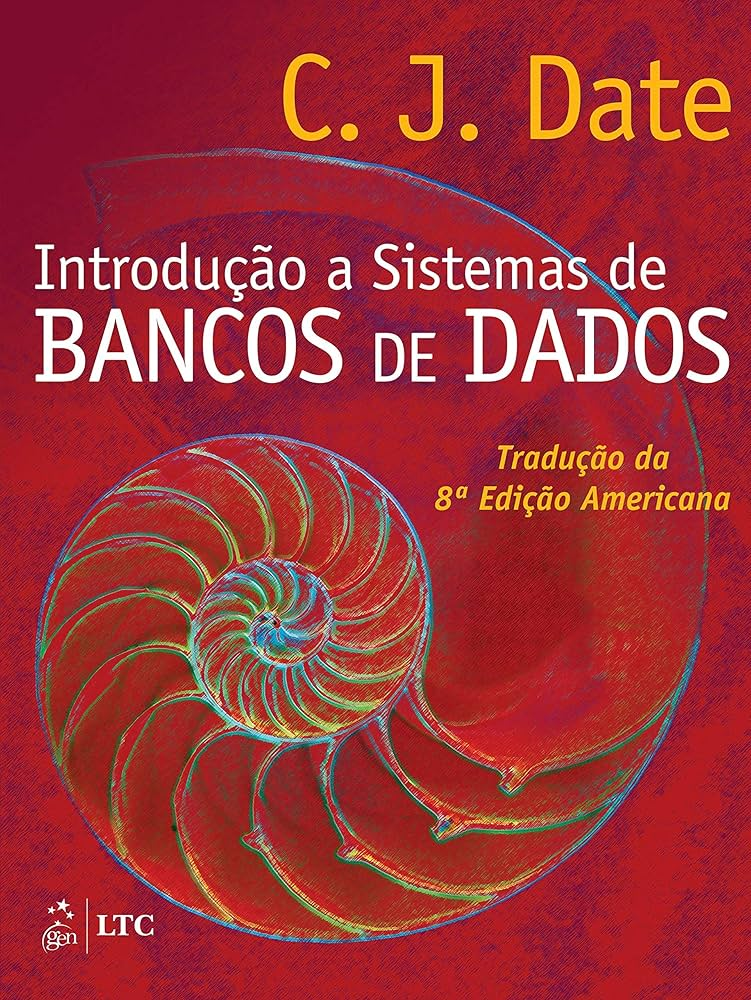
\includegraphics{images/livros/livro1.jpg}

\begin{longtable}[]{@{}
  >{\raggedright\arraybackslash}p{(\columnwidth - 2\tabcolsep) * \real{0.2202}}
  >{\raggedright\arraybackslash}p{(\columnwidth - 2\tabcolsep) * \real{0.7798}}@{}}
\toprule\noalign{}
\endhead
\bottomrule\noalign{}
\endlastfoot
\textbf{Autor(es)} & \begin{minipage}[t]{\linewidth}\raggedright
\subsection{\texorpdfstring{\href{https://en.wikipedia.org/wiki/Christopher_J._Date}{\textbf{Christopher John Date}}}{Christopher John Date}}\label{christopher-john-date}
\end{minipage} \\
\textbf{Editora} & LTC \\
\textbf{Idioma} & Português \\
\textbf{ISBN} & 978-85-352-8445-4 \\
\textbf{Formato} & Capa dura \\
\textbf{Páginas} & 1623 \\
\textbf{Código Biblioteca} & \\
\end{longtable}

\subsection{\texorpdfstring{\href{https://drive.google.com/file/d/0B452rmbcudPSVFdCZ09vVkJUUUd2dlpMNS1vaEczUQ/view?pli=1&resourcekey=0-3MTcHlAYjPX6YSvBQGweUQ}{``\textbf{Projeto de bancos de dados}'' do autor ``Carlos Alberto HEUSER''}}{``Projeto de bancos de dados'' do autor ``Carlos Alberto HEUSER''}}\label{projeto-de-bancos-de-dados-do-autor-carlos-alberto-heuser}

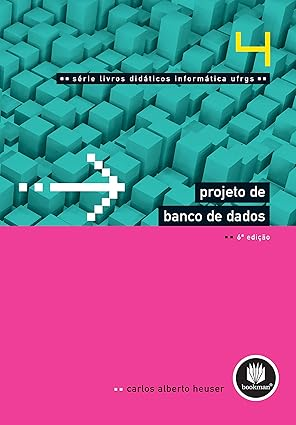
\includegraphics{images/livros/livro2.jpg}

\begin{longtable}[]{@{}
  >{\raggedright\arraybackslash}p{(\columnwidth - 2\tabcolsep) * \real{0.2069}}
  >{\raggedright\arraybackslash}p{(\columnwidth - 2\tabcolsep) * \real{0.7931}}@{}}
\toprule\noalign{}
\endhead
\bottomrule\noalign{}
\endlastfoot
\textbf{Autor(es)} & \begin{minipage}[t]{\linewidth}\raggedright
\subsection{\texorpdfstring{\href{https://www.inf.ufrgs.br/site/docente/carlos-alberto-heuser/}{Carlos Alberto HEUSER}}{Carlos Alberto HEUSER}}\label{carlos-alberto-heuser}
\end{minipage} \\
\textbf{Editora} & Bookman \\
\textbf{Idioma} & Português \\
\textbf{ISBN-10} & 8577803821 \\
\textbf{Formato} & Impresso \\
\textbf{Páginas} & 282 \\
\textbf{Código Biblioteca} & \\
\end{longtable}

\section{Calendário das aulas}\label{calenduxe1rio-das-aulas}

---------------------------------------------------------------------------------------------------------------------------------------

\paragraph{AGOSTO DE 2025}\label{agosto-de-2025}

\begin{longtable}[]{@{}llll@{}}
\toprule\noalign{}
Data & Dia da Semana & Aulas & Conteúdo \\
\midrule\noalign{}
\endhead
\bottomrule\noalign{}
\endlastfoot
04/08/2025 & Segunda-Feira & Aula Inaugural & \\
11/08/2025 & Segunda-Feira & Aula 2 & \\
18/08/2025 & Segunda-Feira & Aula 3 & \\
25/08/2025 & Segunda-Feira & Aula 4 & \\
\end{longtable}

\paragraph{SETEMBRO DE 2025}\label{setembro-de-2025}

\begin{longtable}[]{@{}llll@{}}
\toprule\noalign{}
Data & Dia da Semana & Aulas & Conteúdo \\
\midrule\noalign{}
\endhead
\bottomrule\noalign{}
\endlastfoot
01/09/2025 & Segunda-Feira & Aula 5 & \\
08/09/2025 & Segunda-Feira & Aula 6 & \\
15/09/2025 & Segunda-Feira & NP1 & PROVA \\
22/09/2025 & Segunda-Feira & Aula 7 & \\
29/09/2025 & Segunda-Feira & Aula 8 & \\
\end{longtable}

\paragraph{OUTUBRO DE 2025}\label{outubro-de-2025}

\begin{longtable}[]{@{}llll@{}}
\toprule\noalign{}
Data & Dia da Semana & Aulas & Conteúdo \\
\midrule\noalign{}
\endhead
\bottomrule\noalign{}
\endlastfoot
06/10/2025 & Segunda-Feira & Aula 9 & \\
13/10/2025 & Segunda-Feira & Aula 10 & \\
20/10/2025 & Segunda-Feira & Aula 11 & \\
27/10/2025 & Segunda-Feira & Aula 12 & \\
\end{longtable}

\paragraph{NOVEMBRO DE 2025}\label{novembro-de-2025}

\begin{longtable}[]{@{}llll@{}}
\toprule\noalign{}
Data & Dia da Semana & Aulas & Conteúdo \\
\midrule\noalign{}
\endhead
\bottomrule\noalign{}
\endlastfoot
03/11/2025 & Segunda-Feira & NP2 & PROVA \\
10/11/2025 & Segunda-Feira & & N/A \\
17/11/2025 & Segunda-Feira & SUB & PROVA \\
24/11/2025 & Segunda-Feira & & N/A \\
\end{longtable}

\paragraph{DEZEMBRO DE 2025}\label{dezembro-de-2025}

\begin{longtable}[]{@{}llll@{}}
\toprule\noalign{}
Data & Dia da Semana & Aulas & Conteúdo \\
\midrule\noalign{}
\endhead
\bottomrule\noalign{}
\endlastfoot
01/12/2025 & Segunda-Feira & & N/A \\
08/12/2025 & Segunda-Feira & EXAME & PROVA \\
15/12/2025 & Segunda-Feira & & N/A \\
\end{longtable}

\section{Alunos 2025 - 2o Semestre}\label{alunos-2025---2o-semestre}

---------------------------------------------------------------------------------------------------------------------------------------

\subsection{Campus Chácara Santo Antônio}\label{campus-chuxe1cara-santo-antuxf4nio}

\subsubsection{Turma TI2P40}\label{turma-ti2p40}

\begin{longtable}[]{@{}cc@{}}
\toprule\noalign{}
Matrícula & Nome do aluno \\
\midrule\noalign{}
\endhead
\bottomrule\noalign{}
\endlastfoot
F362BF0 & BRUNO ANTONIO MARQUES \\
R536FA6 & CAIO CESAR BALBINO DA SILVA \\
H6094I1 & DOUGLAS VINICIUS M DOS SANTOS \\
R6607G5 & GABRIEL ROQUE DOS SANTOS \\
R8133G7 & ÍTALO KEVIN RODRIGUES DA SILVA \\
R837AA0 & LUCAS SOUZA RODRIGUES \\
H714419 & MARCOS PAULO CORDEIRO GOES \\
\end{longtable}

\chapter{Aula Inaugural}\label{aula-inaugural}

\subsubsection*{04/08/2025}\label{section}
\addcontentsline{toc}{subsubsection}{04/08/2025}

\subsubsection*{Professor Miguél Suares}\label{professor-miguuxe9l-suares}
\addcontentsline{toc}{subsubsection}{Professor Miguél Suares}

\section{\texorpdfstring{Disciplina: \textbf{Banco de Dados}}{Disciplina: Banco de Dados}}\label{disciplina-banco-de-dados}

\begin{itemize}
\tightlist
\item
  Curso: Gestão em Tecnologia da Informação (GTI)\\
\item
  Período: \textbf{Noturno}\\
\item
  Turma: \textbf{2º semestre de 2025}
\item
  Campus: \textbf{Chácara Santo Antônio}
\end{itemize}

\begin{quote}
``Dados são o novo petróleo.'' -- Clive Humby!
\end{quote}

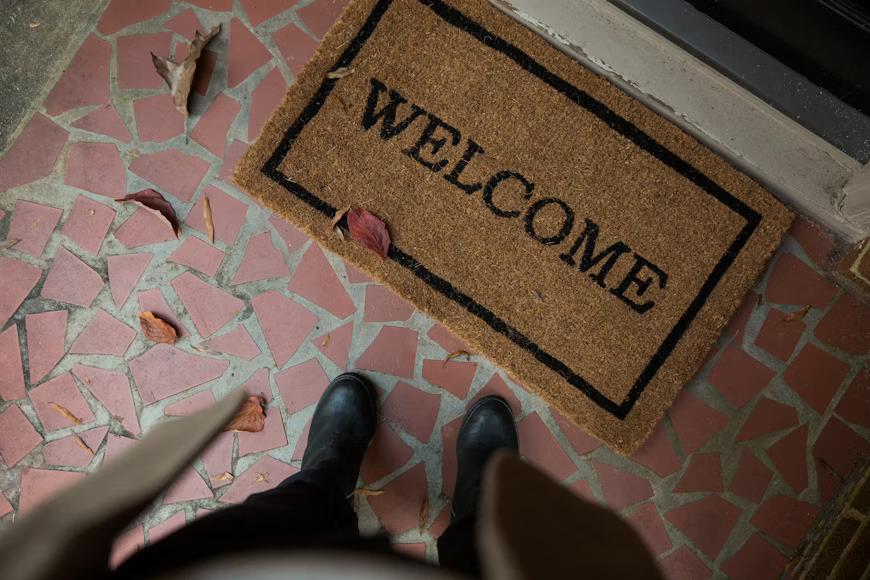
\includegraphics[width=3.125in,height=\textheight]{images/2025-08-04/Boas_Vindas.jpg}

\begin{center}\rule{0.5\linewidth}{0.5pt}\end{center}

\section{👨‍🏫 Sobre o Professor}\label{sobre-o-professor}

\begin{itemize}
\item
  Nome: Prof.~Miguél Suares
\item
  Formação: Mestre em Engenharia da Computação e Energia da Agricultura
\item
  Experiência: +10 anos com bancos de dados relacionais e análise de dados
\item
  Contato: \href{mailto:miguel.penteado@docente.unip.br}{\nolinkurl{miguel.penteado@docente.unip.br}}
\end{itemize}

\begin{center}\rule{0.5\linewidth}{0.5pt}\end{center}

\section{🎯 Objetivos da Disciplina}\label{objetivos-da-disciplina}

\begin{itemize}
\item
  Compreender os fundamentos de bancos de dados
\item
  Modelar dados com diagramas ER
\item
  Implementar e consultar bases de dados com SQL
\item
  Utilizar ferramentas como MySQL, PostgreSQL, QGIS e R
\item
  Desenvolver raciocínio lógico para resolver problemas com dados

  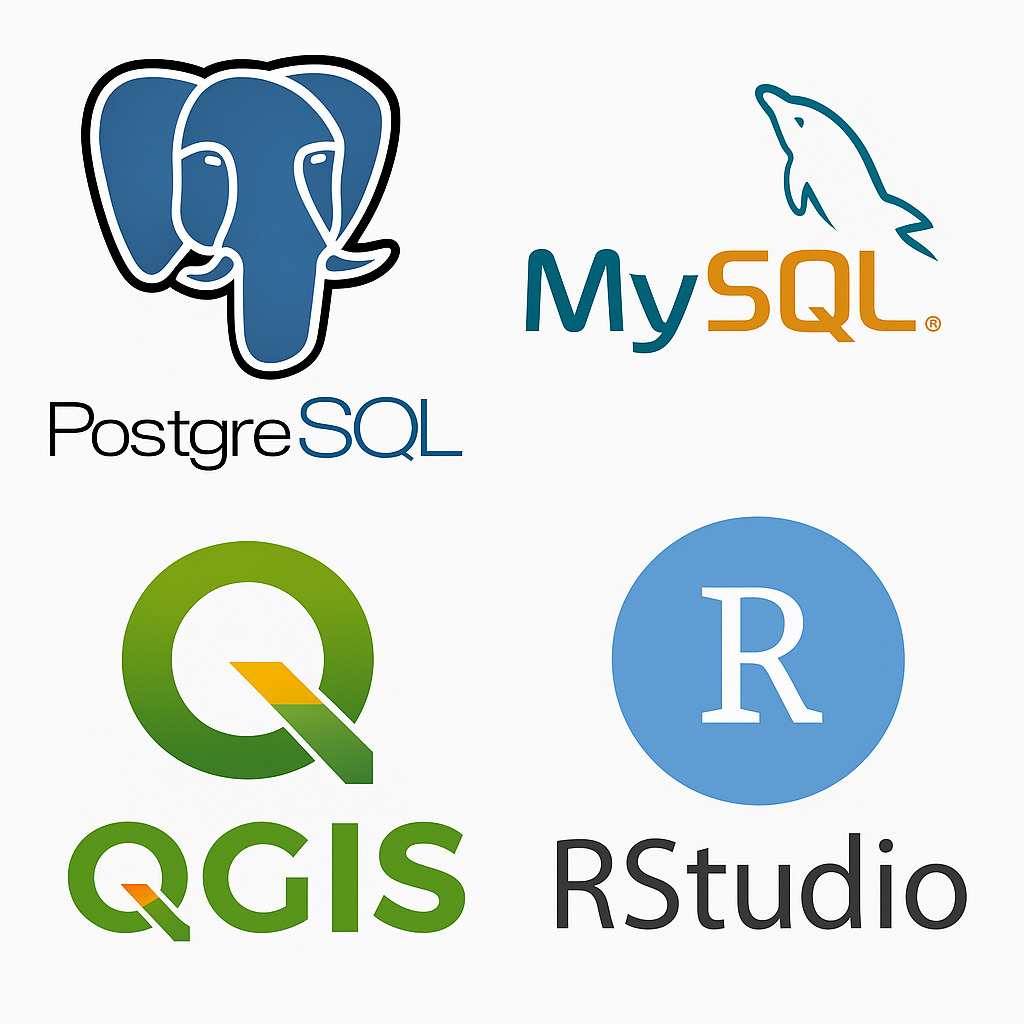
\includegraphics[width=3.47917in,height=\textheight]{images/2025-08-04/logos.jpg}
\end{itemize}

\begin{center}\rule{0.5\linewidth}{0.5pt}\end{center}

\section{📅 Calendário da Disciplina}\label{calenduxe1rio-da-disciplina}

\begin{longtable}[]{@{}lll@{}}
\toprule\noalign{}
Data & Aula & Tema \\
\midrule\noalign{}
\endhead
\bottomrule\noalign{}
\endlastfoot
04/08/2025 & Aula 1 & Aula Inaugural \\
11/08/2025 & Aula 2 & Fundamentos \\
18/08/2025 & Aula 3 & Modelagem e Diagramas \\
25/08/2025 & Aula 4 & Administração e Gerenciamento \\
01/09/2025 & Aula 5 & Aplicação CRUD \\
08/09/2025 & Aula 6 & MySQL \\
15/09/2025 & \textbf{NP1} & \textbf{Prova} \\
22/09/2025 & Aula 7 & Postgres \\
29/09/2025 & Aula 8 & QGIS \\
06/10/2025 & Aula 9 & RStudio \\
13/10/2025 & Aula 10 & Análise I \\
20/10/2025 & Aula 11 & Análise II \\
27/10/2025 & Aula 12 & Análise III \\
03/11/2025 & \textbf{NP2} & \textbf{Prova} \\
\end{longtable}

\begin{center}\rule{0.5\linewidth}{0.5pt}\end{center}

\section{📚 Ementa Resumida}\label{ementa-resumida}

\begin{itemize}
\item
  Introdução a bancos de dados relacionais (RDBMS)
\item
  Modelagem de dados (M.E.R.) e diagramas Entidade Relacionamento (D.E.R.)
\item
  Linguagem SQL: DDL, DML, DCL
\item
  Ferramentas: MySQL, PostgreSQL
\item
  Visualização geoespacial (QGIS)
\item
  Análise e exploração de dados (R e RStudio)

  \includegraphics[width=3.44792in,height=\textheight]{images/2025-08-04/modelagem.jpg}
\end{itemize}

\begin{center}\rule{0.5\linewidth}{0.5pt}\end{center}

\section{📝 Avaliação}\label{avaliauxe7uxe3o}

\begin{itemize}
\tightlist
\item
  \textbf{Provas (NP1 + NP2)}
\item
  \textbf{Prova Substitutiva}
\item
  \textbf{Exame}
\end{itemize}

\begin{center}\rule{0.5\linewidth}{0.5pt}\end{center}

\section{🛠️ Ferramentas da Disciplina}\label{ferramentas-da-disciplina}

\begin{itemize}
\tightlist
\item
  \textbf{Servidores de Banco de Dados}: MySQL, PostgreSQL
\item
  \textbf{Servidores de Banco de Dados}: pgAdmin, MySQL Workbench, DBeaver\\
\item
  \textbf{Geoprocessamento}: QGIS\\
\item
  \textbf{Análise de Dados}: R + RStudio\\
\item
  \textbf{Versionamento e Organização}: GitHub, Teams
\end{itemize}

\begin{center}\rule{0.5\linewidth}{0.5pt}\end{center}

\section{📌 Expectativas e Regras}\label{expectativas-e-regras}

\begin{itemize}
\tightlist
\item
  Pontualidade e entrega de atividades no prazo
\item
  Trabalhos devem ser originais (sem plágio)
\item
  Participação ativa nas discussões e práticas
\item
  Uso responsável das ferramentas
\item
  Respeito e colaboração entre colegas
\end{itemize}

\begin{center}\rule{0.5\linewidth}{0.5pt}\end{center}

\section{💡 Dicas para Mandar Bem}\label{dicas-para-mandar-bem}

\begin{itemize}
\tightlist
\item
  Faça os exercícios logo após a aula
\item
  Participe das práticas com base real
\item
  Mantenha o repositório do projeto atualizado
\item
  Refaça consultas SQL até entender
\item
  Teste e documente suas soluções
\end{itemize}

\begin{center}\rule{0.5\linewidth}{0.5pt}\end{center}

\section{🙌 Encerramento}\label{encerramento}

\section{Estamos prontos?}\label{estamos-prontos}

📧 Dúvidas? Estou à disposição\\
📊 Vamos construir conhecimento juntos!

\begin{quote}
Próxima aula: \textbf{Fundamentos de Banco de Dados} -- 11/08/2025
\end{quote}

\chapter{Fundamentos de Sistemas de Bancos de Dados}\label{fundamentos-de-sistemas-de-bancos-de-dados}

\subsubsection*{11/08/2025}\label{section-1}
\addcontentsline{toc}{subsubsection}{11/08/2025}

\subsubsection*{Professor Miguél Suares}\label{professor-miguuxe9l-suares-1}
\addcontentsline{toc}{subsubsection}{Professor Miguél Suares}

\begin{center}\rule{0.5\linewidth}{0.5pt}\end{center}

\section{O início : Edgar Frank ``Ted'' Codd (19/08/1923 -- 18/04/2003)}\label{o-inuxedcio-edgar-frank-ted-codd-19081923-18042003}

\begin{itemize}
\item
  Nome: Professor Codd - Matemático da IBM

  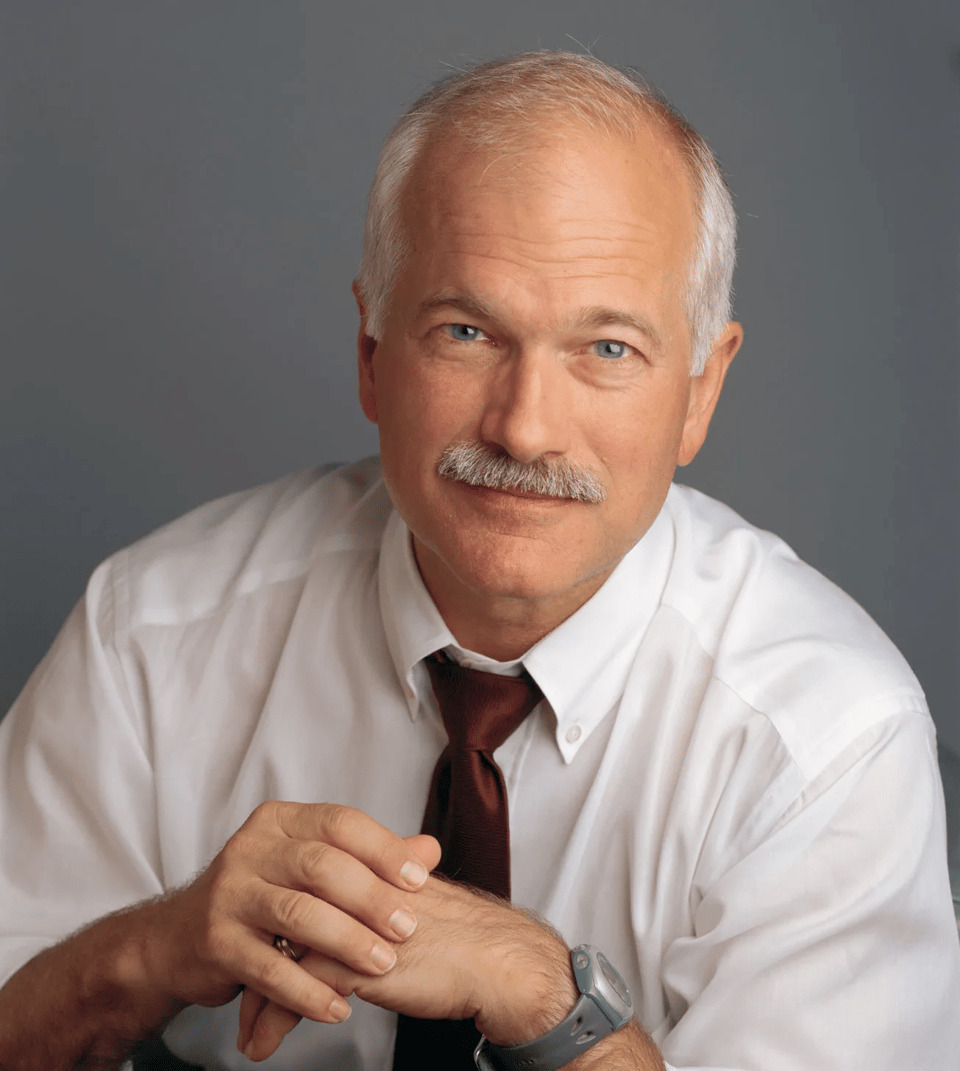
\includegraphics[width=1.39583in,height=\textheight]{images/2025-08-11/01-codd.jpg}
\item
  1965: Cria modelo relacional nos tempos da IBM/NASA/Projeto Apolo
\end{itemize}

\includegraphics[width=3.47917in,height=\textheight]{images/2025-08-11/modelagem.jpg}

\begin{itemize}
\item
  1969: Codd não é levado a sério
\item
  1970: Publica a teoria relacional nas universidades (Berkley, Califórnia)
\end{itemize}

\begin{center}\rule{0.5\linewidth}{0.5pt}\end{center}

\section{Anos 1970: IBM entra no Modelo relacional: SystemR e SEQUEL/SQL}\label{anos-1970-ibm-entra-no-modelo-relacional-systemr-e-sequelsql}

\begin{itemize}
\item
  1970: IBM entende a importância do modelo de Codd
\item
  1971: Como Codd publica o conhecimento, o projeto vai para \emph{Raymond Francis Boyce}

  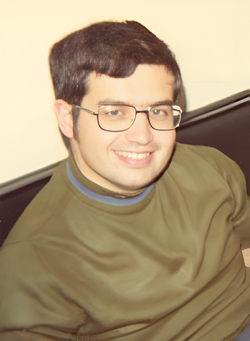
\includegraphics[width=1.4375in,height=\textheight]{images/2025-08-11/05-Boyce.png}
\item
  1974: Donald D. Chamberlin e \emph{Raymond Francis Boyce} criam a SQL na IBM
\item
  1973: \emph{Raymond Francis Boyce} criam o SystemR (Banco Relacional da IBM)
\item
  Codd continua publicando artigos sobre modelo relacional
\item
  1977: Ex-alunos prof Michael StoneBraker fundam a (Relational Inc) ORACLE ``copiando'' o SystemR da IBM.

  
\includegraphics[width=1.375in,height=\textheight]{images/2025-08-11/06-oracle.png}
\end{itemize}

\begin{center}\rule{0.5\linewidth}{0.5pt}\end{center}

\section{Anos 1970: Prof Codd inspira Prof StoneBraker: BANCO INGRES}\label{anos-1970-prof-codd-inspira-prof-stonebraker-banco-ingres}

\begin{itemize}
\item
  1974: Michael StoneBraker começa projeto INGRES na Universidade de Berkley

  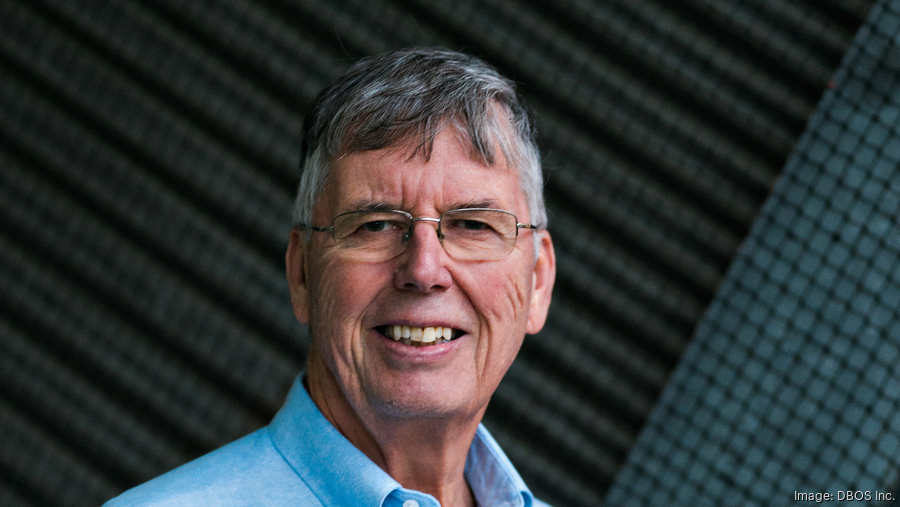
\includegraphics[width=2.10417in,height=\textheight]{images/2025-08-11/07-Michael_StoneBraker.png}
\item
  1976: Nasce o INGRES, pai de muitos Bancos de Dados Modernos.

  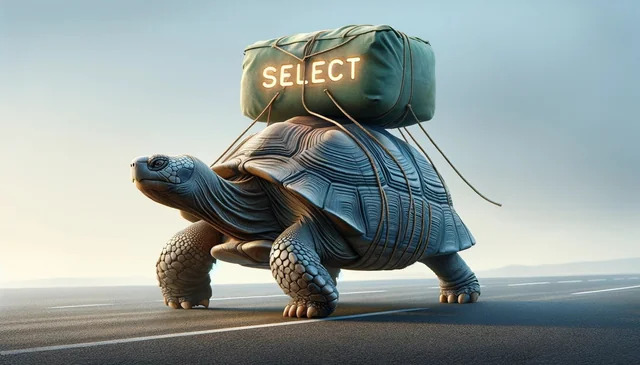
\includegraphics[width=1.80208in,height=\textheight]{images/2025-08-11/03-ingress-1.0.jpg}
\item
  1976: INGRES nasce com linguagem prórpia, o QUEL, ao invés do SQL
\item
  INGRESS cria a empresa Relational INC
\item
  Ex-funcionários (alunos) da Relational Inc fundam a SYBASE.
\end{itemize}

\begin{center}\rule{0.5\linewidth}{0.5pt}\end{center}

\section{Anos 1980: INGRES (SEMI-LIVRE) vs IBM System R ( pago ) vs ORACLE}\label{anos-1980-ingres-semi-livre-vs-ibm-system-r-pago-vs-oracle}

\begin{itemize}
\item
  1982 IBM transforma SystemR em IBM DB2.
\item
  1984 Ex-funcionários (alunos) da Relational Inc fundam a SYBASE.

  
\includegraphics[width=2.67708in,height=\textheight]{images/2025-08-11/08-sybase.png}
\item
  1985: SoneBraker cria o PostGRES (Banco de Dados Objeto-Relacional)
\item
  1986: INGRES perde para a ORACLE no mercado de SGBDs
\item
  1989: SQL vira padrão ANSI e padrão ISO
\end{itemize}

\begin{center}\rule{0.5\linewidth}{0.5pt}\end{center}

\section{Anos 1990: MySQL e POSTGRES que vira POSTGRESQL}\label{anos-1990-mysql-e-postgres-que-vira-postgresql}

\begin{itemize}
\item
  1993: O SYBASE SQL Server é portado para o Windows NT 4.0
\item
  1994: Fim do relacionamento entre Microsoft e SYBASE: nasce o MS-SQL Server
\item
  1994: \textbf{Andrew Yu} e \textbf{Jolly Chen} Adicionam SQL ao POSTGRES: nasce o \textbf{PostgreSQL}

  
\includegraphics[width=1.46875in,height=\textheight]{images/2025-08-11/10-postgresql.png}
\item
  1994: David Axmark, Allan Larsson e Michael ``Monty'' Widenius criam o MySQL.

  
\includegraphics[width=1.36458in,height=\textheight]{images/2025-08-11/09-mysql.png}
\item
  1997: Nasce o postgreSQL 6.0
\item
  1998: Carlo Strozzi - Modelo Não-SQL (conceito de SGBDs que não usam interface SQL)
\end{itemize}

\begin{center}\rule{0.5\linewidth}{0.5pt}\end{center}

\section{Anos 2000: Sybase eo No-SQL}\label{anos-2000-sybase-eo-no-sql}

\begin{itemize}
\item
  2003 - Doug Cutting e Mike Cafarella, projeto \emph{Hadoop} baeado no documento \emph{Google File System}
\item
  2007 - 10gen (MongoDB Inc) inicia o projeto MongoDB (Não SQL)

  
\includegraphics[width=2.70833in,height=\textheight]{images/2025-08-11/11-mongodb.png}
\item
  2007 - Avinash Lakshman do facebook disponibiliza o Apache Cassandra (Não SQL)

  
\includegraphics[width=1.3125in,height=\textheight]{images/2025-08-11/12-cassandra.png}
\item
  2008 - BIG DATA Lançado o Apache HADOOP e o Apache Hive (emulador SQL)

  
\includegraphics[width=4.59375in,height=\textheight]{images/2025-08-11/13-hadoop.png}BIG

  
\includegraphics[width=1.44792in,height=\textheight]{images/2025-08-11/14-Apache_Hive.png}
\end{itemize}

\begin{center}\rule{0.5\linewidth}{0.5pt}\end{center}

\chapter{Modelagem de Bancos de Dados}\label{modelagem-de-bancos-de-dados}

\subsubsection*{18/08/2025}\label{section-2}
\addcontentsline{toc}{subsubsection}{18/08/2025}

\subsubsection*{Professor Miguél Suares}\label{professor-miguuxe9l-suares-2}
\addcontentsline{toc}{subsubsection}{Professor Miguél Suares}

\section{Introdução: Visitando a teoria de Bancos de Dados}\label{introduuxe7uxe3o-visitando-a-teoria-de-bancos-de-dados}

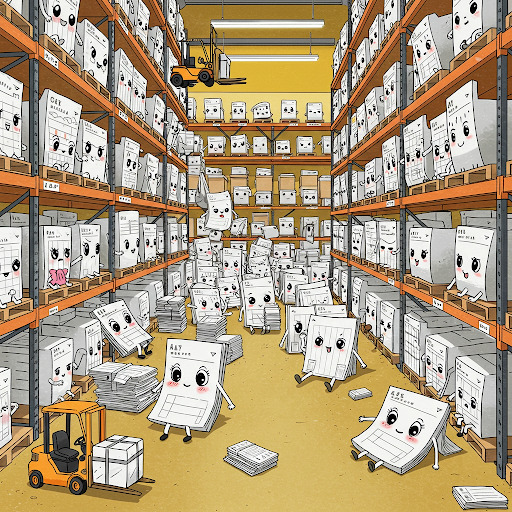
\includegraphics[width=4.70833in,height=\textheight]{images/5-bi/01-banco-de-dados.jpg}

\begin{quote}
\textbf{Banco de Dados} Um banco de dados é uma coleção compartilhada de dados logicamente relacionados, projetada para atender às necessidades informacionais de uma organização. - \emph{DATE, C. J. An Introduction to Database Systems. 8. ed.~Boston: Addison-Wesley, 2003}.
\end{quote}

Ou seja, alguns pontos-chave da definição de Date:

\begin{itemize}
\item
  ``Coleção de dados \ldots{}'' → não é um conjunto de arquivos soltos, mas dados organizados.
\item
  ``Compartilhada \ldots{}'' → não pertence a apenas um usuário ou aplicação; é usada por vários.
\item
  ``Dados logicamente relacionados \ldots{}'' → os dados têm um relacionamento semântico, não são apenas agrupamentos arbitrários.
\item
  ``Projetada para atender necessidades \ldots{}'' → o banco existe para suportar os processos de uma organização (consultas, relatórios, controle, tomada de decisão).
\end{itemize}

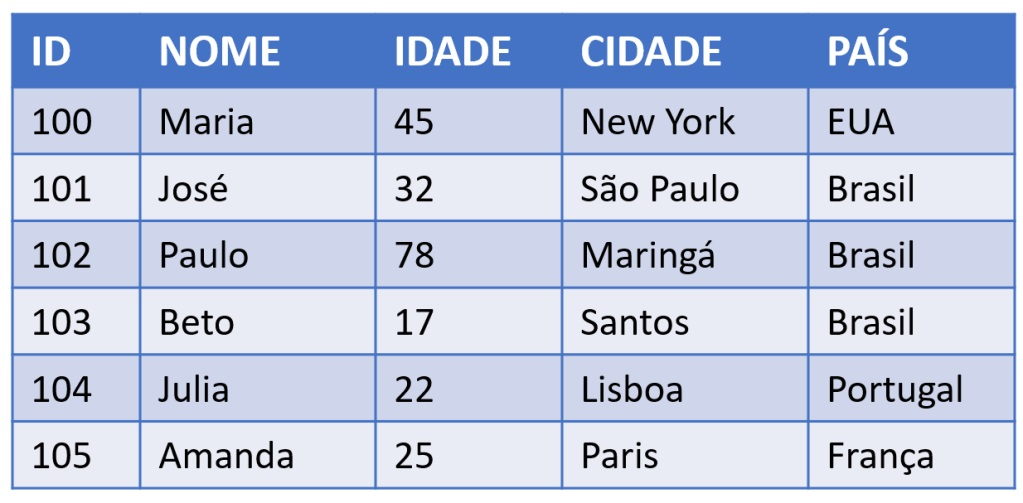
\includegraphics{images/5-bi/07-tabela_relacional.jpg}

\begin{quote}
\textbf{Banco de Dados Relacional} Um banco de dados relacional é um banco de dados baseado em um modelo de dados relacional, no qual os dados são representados como um conjunto de relações (tabelas), e cada relação consiste em tuplas (linhas) e atributos (colunas). - \emph{SILBERSCHATZ, Abraham; KORTH, Henry F.; SUDARSHAN, S. Database System Concepts. 6. ed.~New York: McGraw-Hill, 2010.}
\end{quote}

Agora, alguns pontos-chave da definição de \emph{Abraham Silberschatz} :

\begin{itemize}
\item
  Base no modelo relacional de Codd (1970).
\item
  Dados representados em tabelas (relações).
\item
  Cada tabela é composta de tuplas (linhas) e atributos (colunas).
\item
  Integridade garantida por restrições (chaves, integridade referencial, domínio de atributos).
\item
  Manipulação feita por linguagens relacionais (álgebra relacional, cálculo relacional, SQL).
\end{itemize}

O Banco de Dados Relacional organiza as informações em \textbf{tabelas bidiomensionais} constituídas de \textbf{linhas e colunas} chamadas e essas tabelas recebem o nome de \textbf{relações}. Cada \textbf{relação} possui um \textbf{campo-chave} que confere identificação exclusiva a cada registro da tabela.

\section{Modelo Matemático de um Banco de Dados}\label{modelo-matemuxe1tico-de-um-banco-de-dados}

Considere um Banco de Dados para representar, com consistência Matemática os
funcionários e Departamentos de uma Empresa.

\subsection{Podemos representa-lo matemáticamente utilizando a teoria dos conjuntos}\label{podemos-representa-lo-matemuxe1ticamente-utilizando-a-teoria-dos-conjuntos}

\begin{figure}
\centering
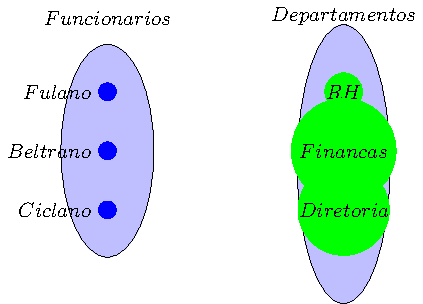
\includegraphics{2025-GTI-Sem-BancoDeDados_files/figure-latex/tikz-diagrama0-1.pdf}
\caption{\label{fig:tikz-diagrama0}Diagrama de Montadoras, Veículos e Proprietários}
\end{figure}

\subsubsection{\texorpdfstring{Edgard F Cood explica em sua obra ``A Relational Model of Data for Large Shared Data Banks'' como definir uma Banco de Dados compartilhado \emph{matemáticamente}}{Edgard F Cood explica em sua obra ``A Relational Model of Data for Large Shared Data Banks'' como definir uma Banco de Dados compartilhado matemáticamente}}\label{edgard-f-cood-explica-em-sua-obra-a-relational-model-of-data-for-large-shared-data-banks-como-definir-uma-banco-de-dados-compartilhado-matemuxe1ticamente}

\begin{quote}
Um banco de dados relacional é um banco de dados no qual todos os dados são representados por meio de relações (matematicamente, conjuntos de tuplas), e todas as operações sobre os dados são baseadas em operadores formais do cálculo relacional e da álgebra relacional. - \emph{A Relational Model of Data for Large Shared Data Banks'' (Communications of the ACM, vol.~13, n.~6, pp.~377--387, 1970).}
\end{quote}

\subsection{Então para podemos relacionar estes dois conjuntos (Funcionários e Departamentos) utilizando a Teoria das Funções}\label{entuxe3o-para-podemos-relacionar-estes-dois-conjuntos-funcionuxe1rios-e-departamentos-utilizando-a-teoria-das-funuxe7uxf5es}

\$\$

f(x) = Y

\$\$

\$\$

F(Funcionário) = Departamento

\$\$

\begin{figure}
\centering
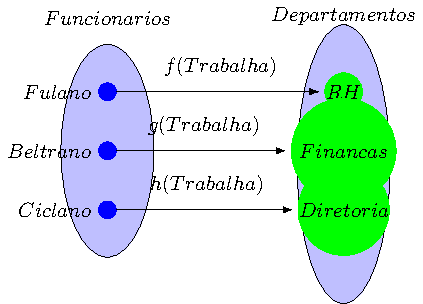
\includegraphics{2025-GTI-Sem-BancoDeDados_files/figure-latex/tikz-diagrama10-1.pdf}
\caption{\label{fig:tikz-diagrama10}Diagrama de Montadoras, Veículos e Proprietários}
\end{figure}

Mas vai ficar faltando como representar os atributos nesse modelo (colunas das tabelas):

Ainda, é necessário acrescentar algumas regras de integridade a representação;

\section{Modelo Lógico de Banco de Dados}\label{modelo-luxf3gico-de-banco-de-dados}

\subsection{Modelo Conceitual ``Entidade Relacionamento'' de Banco de Dados}\label{modelo-conceitual-entidade-relacionamento-de-banco-de-dados}

O Modelo Entidade-Relacionamento (MER), proposto por Peter Chen em 1976, é uma ferramenta fundamental na modelagem de dados. É um modelo de dados de alto nível que descreve a estrutura conceitual de um banco de dados. O Modelo Entidade-Relacionamento (MER) é representado graficamente através de um DER (Diagrama Entidade-Relacionamento).

É utilizado para projetar Bancos de Dados Relacionais a partir de entrevistas onde se descreve as informações que se deseja armazenar de forma consistente. Exemplo:

``\emph{Desenhe um diagrama entidade-relacionamento DER contendo as entidades funcionarios e departamentos. A entidade ''funcionários'' possui os atributos ''nome'' e ''CPF''. A entidade ''Departamentos'' possui os atributos ''Nome'' e ''sigla''. O atributo ''CPF'' é chave primária da entidade ''Funcionários''. O atributo ''sigla'' é chave primária da entidade ''Departamentos''. As entidades ''Funcionários'' e ''Departamentos'' se relacionam através de um relacionamento chamado ''Pertence''}.''

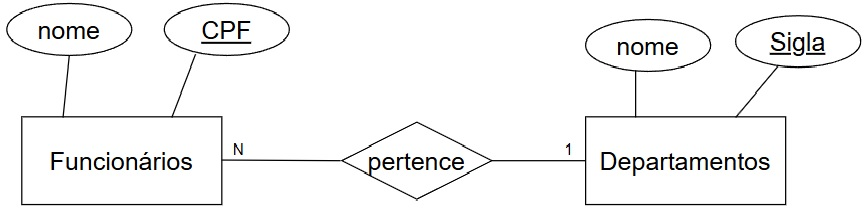
\includegraphics{images/5-bi/02-Modelo-Entidade-Relacionamento.jpg}

Segundo Laudon

\begin{quote}
\textbf{Diagrama Entidade/Relacionamento (DER)} é uma representação esquemática utilizada para entender as relações entre as tabelas de um banco de dados relacional. {[}{[}1{]} - LAUDON, Kenneth C.; LAUDON, Jane P. *Sistemas de informação gerenciais*. 11. ed.~São Paulo: Pearson Education do Brasil, 2010. p.~180.{]}
\end{quote}

\subsection{Composição e Significado do Diagrama Entidade Relacionamento (DER)}\label{composiuxe7uxe3o-e-significado-do-diagrama-entidade-relacionamento-der}

\begin{longtable}[]{@{}
  >{\centering\arraybackslash}p{(\columnwidth - 4\tabcolsep) * \real{0.1613}}
  >{\centering\arraybackslash}p{(\columnwidth - 4\tabcolsep) * \real{0.3871}}
  >{\centering\arraybackslash}p{(\columnwidth - 4\tabcolsep) * \real{0.4409}}@{}}
\toprule\noalign{}
\endhead
\bottomrule\noalign{}
\endlastfoot
\textbf{Nome} & \textbf{Desenho} & \textbf{Significado} \\
Entidade & 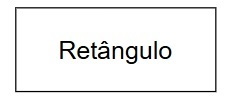
\includegraphics{images/5-bi/03-retangulo.jpg} & Representa uma tabela e é identificada

no texto por um \textbf{substantivo}. \\
\end{longtable}

\begin{longtable}[]{@{}
  >{\centering\arraybackslash}p{(\columnwidth - 4\tabcolsep) * \real{0.1061}}
  >{\centering\arraybackslash}p{(\columnwidth - 4\tabcolsep) * \real{0.3485}}
  >{\centering\arraybackslash}p{(\columnwidth - 4\tabcolsep) * \real{0.5379}}@{}}
\toprule\noalign{}
\endhead
\bottomrule\noalign{}
\endlastfoot
\textbf{Nome} & \textbf{Desenho} & \textbf{Significado} \\
Atributo & 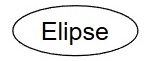
\includegraphics[width=1.89583in,height=\textheight]{images/5-bi/05-elipse.jpg} & Representa uma coluna e é identificada no texto por um \textbf{adjetivo}. \\
\end{longtable}

\begin{longtable}[]{@{}
  >{\centering\arraybackslash}p{(\columnwidth - 4\tabcolsep) * \real{0.1491}}
  >{\centering\arraybackslash}p{(\columnwidth - 4\tabcolsep) * \real{0.4123}}
  >{\centering\arraybackslash}p{(\columnwidth - 4\tabcolsep) * \real{0.4298}}@{}}
\toprule\noalign{}
\endhead
\bottomrule\noalign{}
\endlastfoot
\textbf{Nome} & \textbf{Desenho} & \textbf{Significado} \\
Relacionamento & 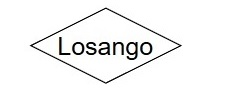
\includegraphics[width=1.92708in,height=\textheight]{images/5-bi/04-losango.jpg} & Representa uma \textbf{Referência} e é identificada

no texto por um \textbf{Verbo}. \\
\end{longtable}

\section{Modelo Físico de Banco de Dados}\label{modelo-fuxedsico-de-banco-de-dados}

\subsection{Geração do modelo Físico para aplica-lo ao SGBD (Sistema de Gerenciamento de Banco de Dados):}\label{gerauxe7uxe3o-do-modelo-fuxedsico-para-aplica-lo-ao-sgbd-sistema-de-gerenciamento-de-banco-de-dados}

Uma vez que o modelo conceitual seja gerado, o analista pode mapea-lo para um ``modelo físico'' onde se mapeiam chaves primárias e chaves forasteiras nas tabelas.

Após a geração do modelo físico pode-se gerar o SQL que monta a estrutura do Banco de Dados.

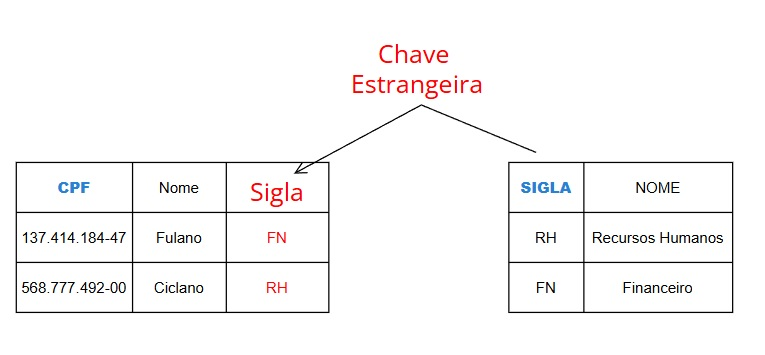
\includegraphics{images/5-bi/06-modelo_fisico.jpg}

\subsection{Código SQL - Implementação do Modelo Físico}\label{cuxf3digo-sql---implementauxe7uxe3o-do-modelo-fuxedsico}

\begin{Shaded}
\begin{Highlighting}[]
\CommentTok{{-}{-} Exemplo testado e gerado no SGBD Postgres versão 15}

\CommentTok{{-}{-} Tabela Funcionários}
\KeywordTok{CREATE} \KeywordTok{TABLE} \ControlFlowTok{IF} \KeywordTok{NOT} \KeywordTok{EXISTS} \OtherTok{"public"}\NormalTok{.funcionarios}
\NormalTok{(}
\NormalTok{    cpf bigint }\KeywordTok{NOT} \KeywordTok{NULL}\NormalTok{,}
\NormalTok{    nome }\DataTypeTok{varchar}\NormalTok{(}\DecValTok{200}\NormalTok{)}
\NormalTok{);}

\CommentTok{{-}{-} Tabela Departamentos}

\KeywordTok{CREATE} \KeywordTok{TABLE} \ControlFlowTok{IF} \KeywordTok{NOT} \KeywordTok{EXISTS} \OtherTok{"public"}\NormalTok{.departamentos}
\NormalTok{(}
\NormalTok{    sigla }\DataTypeTok{integer} \KeywordTok{NOT} \KeywordTok{NULL}\NormalTok{,}
\NormalTok{    nome }\DataTypeTok{varchar}\NormalTok{(}\DecValTok{200}\NormalTok{)}
\NormalTok{);}

\CommentTok{{-}{-} Definindo a coluna "cpf" da tabela "funcionários" como chave primária}
\KeywordTok{alter} \KeywordTok{table} \OtherTok{"public"}\NormalTok{.funcionarios }\KeywordTok{add} \KeywordTok{constraint} \OtherTok{"chave\_primaria\_funcionarios"} \KeywordTok{primary} \KeywordTok{key}\NormalTok{ (cpf);}

\CommentTok{{-}{-} Definindo a coluna "sigla"" da tabela "departamentos" como chave primária}
\KeywordTok{alter} \KeywordTok{table} \OtherTok{"public"}\NormalTok{.departamentos }\KeywordTok{add} \KeywordTok{constraint} \OtherTok{"chave\_primaria\_departamentos"} \KeywordTok{primary} \KeywordTok{key}\NormalTok{ (sigla);}

\CommentTok{{-}{-} Gerando a integridade referêncial }
\CommentTok{{-}{-} Importando a chave primária da tabela "departamentos" como "chave estrangeira"}
\CommentTok{{-}{-} na tabela "funcionários"}

\CommentTok{{-}{-} primeiro adiciona{-}se a coluna estrageira "sigla" que é coluna originalmente }
\CommentTok{{-}{-} pertencente a tabela departamentos}
\KeywordTok{alter} \KeywordTok{table} \OtherTok{"public"}\NormalTok{.funcionarios }\KeywordTok{add} \KeywordTok{column}\NormalTok{ sigla }\DataTypeTok{integer}\NormalTok{;}

\CommentTok{{-}{-} finalmente conecte a coluna sigla a chave primária da tabela "departamento"}
\CommentTok{{-}{-} criando então uma chave estrageira na tabela "funcionários".}
\KeywordTok{alter} \KeywordTok{table} \OtherTok{"public"}\NormalTok{.funcionarios }\KeywordTok{add} \KeywordTok{constraint} \OtherTok{"Chave\_estrangeira\_Departamento\_funcionarios"} \KeywordTok{foreign} \KeywordTok{key}\NormalTok{ (sigla) }\KeywordTok{references} \OtherTok{"public"}\NormalTok{.departamentos(sigla);}
\end{Highlighting}
\end{Shaded}

\section{EXEMPLO: MONTADORA}\label{exemplo-montadora}

\subsection{Modelo Matemático}\label{modelo-matemuxe1tico}

Construa um Banco de Dados com suporte a consistência das informações. Utilize para isso o modelo Relacional. Precisamos armazenar as informações dos Veículos, Montadoras e Proprietários;

\subsubsection{Representação Matemática em Conjuntos e seus Elementos :}\label{representauxe7uxe3o-matemuxe1tica-em-conjuntos-e-seus-elementos}

\begin{figure}
\centering
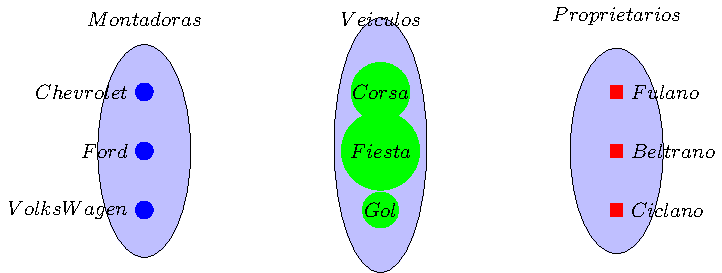
\includegraphics{2025-GTI-Sem-BancoDeDados_files/figure-latex/tikz-diagrama1-1.pdf}
\caption{\label{fig:tikz-diagrama1}Diagrama de Montadoras, Veículos e Proprietários}
\end{figure}

\subsubsection{Gerando os Relacionamentos ``Matemáticamente'' - (Teoria das Funções, Domínios e Imagens):}\label{gerando-os-relacionamentos-matemuxe1ticamente---teoria-das-funuxe7uxf5es-domuxednios-e-imagens}

\begin{figure}
\centering
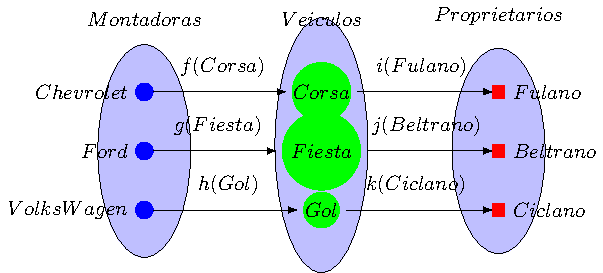
\includegraphics{2025-GTI-Sem-BancoDeDados_files/figure-latex/tikz-diagrama2-1.pdf}
\caption{\label{fig:tikz-diagrama2}Diagrama de Montadoras, Veículos e Proprietários}
\end{figure}

\section{Normalização em Bancos de Dados Relaionais}\label{normalizauxe7uxe3o-em-bancos-de-dados-relaionais}

\subsection{Tabela Desnormalizada}\label{tabela-desnormalizada}

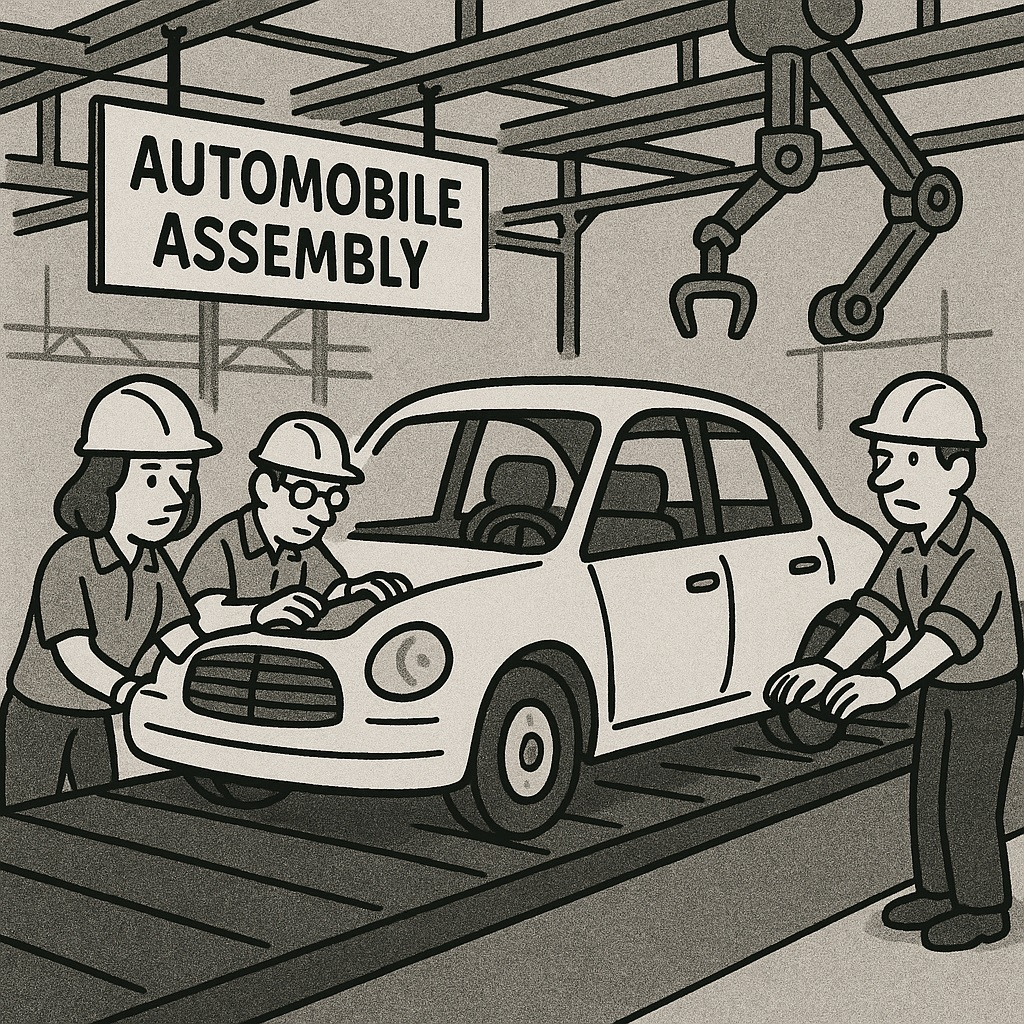
\includegraphics[width=3.57292in,height=\textheight]{images/5-bi/01-montadora.jpg}

Considere a tabela Veículos abaixo:

\begin{longtable}[]{@{}cc@{}}
\toprule\noalign{}
Modelo & Montadora \\
\midrule\noalign{}
\endhead
\bottomrule\noalign{}
\endlastfoot
Strada & Fiat \\
Mobi & Fiat \\
Pulse & Fiat \\
Onix & Chevrolet \\
Tracker & Chevrolet \\
Onix Plus & Chevrolet \\
Polo & Volkswagen \\
Nivus & Volkswagen \\
T-Cross & Volkswagen \\
HB20 & Hyundai \\
Creta & Hyundai \\
\end{longtable}

Separamos o conjunto de elemntos \emph{Montadoras} e \emph{Modelos}.

\begin{longtable}[]{@{}cc@{}}
\toprule\noalign{}
MontadoraID & Montadora \\
\midrule\noalign{}
\endhead
\bottomrule\noalign{}
\endlastfoot
1 & Fiat \\
2 & Chevrolet \\
3 & Volkswagen \\
4 & Hyundai \\
\end{longtable}

\begin{longtable}[]{@{}cc@{}}
\toprule\noalign{}
ModeloID & Modelo \\
\midrule\noalign{}
\endhead
\bottomrule\noalign{}
\endlastfoot
101 & Strada \\
102 & Mobi \\
103 & Pulse \\
201 & Onix \\
202 & Tracker \\
203 & Onix Plus \\
301 & Polo \\
302 & Nivus \\
303 & T-Cross \\
401 & HB20 \\
402 & Creta \\
\end{longtable}

\begin{quote}
O processo de fragmentar agrupamentos complexos de dados e simplifica-los a fim de minimizar redundâncias e economizar espaço no Banco de Dados Relacional é chamado de \textbf{NORMALIZAÇÃO.} {[}{[}1{]} - LAUDON, Kenneth C.; LAUDON, Jane P. *Sistemas de informação gerenciais*. 11. ed.~São Paulo: Pearson Education do Brasil, 2010. p.~180.{]}
\end{quote}

Mas Como indicar que cada elemento da tabela ``Modelo'' está associado a um elemento da tabela ``Montadora'' ?

\subsection{Tabela Normalizada}\label{tabela-normalizada}

Considere as tabelas abaixo:

\begin{longtable}[]{@{}
  >{\centering\arraybackslash}p{(\columnwidth - 2\tabcolsep) * \real{0.2361}}
  >{\centering\arraybackslash}p{(\columnwidth - 2\tabcolsep) * \real{0.5417}}@{}}
\toprule\noalign{}
\begin{minipage}[b]{\linewidth}\centering
MontadoraID
\end{minipage} & \begin{minipage}[b]{\linewidth}\centering
Montadora
\end{minipage} \\
\midrule\noalign{}
\endhead
\bottomrule\noalign{}
\endlastfoot
1 & Fiat \\
2 & Chevrolet \\
3 & Volkswagen \\
4 & Hyundai \\
\end{longtable}

\begin{longtable}[]{@{}ccc@{}}
\toprule\noalign{}
ModeloID & Modelo & MontadoraID \\
\midrule\noalign{}
\endhead
\bottomrule\noalign{}
\endlastfoot
101 & Strada & 1 \\
102 & Mobi & 1 \\
103 & Pulse & 1 \\
201 & Onix & 2 \\
202 & Tracker & 2 \\
203 & Onix Plus & 2 \\
301 & Polo & 3 \\
302 & Nivus & 3 \\
303 & T-Cross & 3 \\
401 & HB20 & 4 \\
402 & Creta & 4 \\
\end{longtable}

Repare que:

\begin{itemize}
\item
  É possível identificar que não existem montadoras repetidas na tabela ``Montadoras'';
\item
  É possível identificar que não existem modelos repetidos na tabela ``Montadoras'';
\end{itemize}

A coluna (atributo) \textbf{ModeloID} é a \textbf{chave primária} da tabela \textbf{Modelos.} A coluna (atributo) \textbf{MontadoraID} é a \textbf{chave primária} da tabela \textbf{Montadoras.}

Na tabela \textbf{Modelos}, a coluna \textbf{MontadoraID}, acrescentada a tabela Modelos representa a ligação de cada elemento da tabela Modelos e Montadoras. Essa coluna ``importada'' da tabela Montadoras para a tabela Modelos se chama \textbf{chave estrangeira}.

\section{Exercícios}\label{exercuxedcios}

1- Construa um projeto Banco de Dados Relacional para uma universidade. Mapeie
no seu Banco de Dados Disciplinas, Professores e Alunos.
Para isso, faça o modelo ``matemático'', o Modelo Lógico e o Modelo Físico com SQL.

\section{Referências}\label{referuxeancias}

\textbf{DATE}, C. J. \textbf{An Introduction to Database Systems.} 8. ed.~Boston: Addison-Wesley, 2003.

\textbf{SILBERSCHATZ}, Abraham; KORTH, Henry F.; SUDARSHAN, S. \textbf{Database System Concepts.} 6. ed.~New York: McGraw-Hill, 2010.

\textbf{CODD}, E. F. \textbf{A Relational Model of Data for Large Shared Data Banks.} Communications of the ACM, New York, v. 13, n.~6, p.~377--387, 1970.

\chapter{Administração e Gerenciamento de Bancos de Dados}\label{administrauxe7uxe3o-e-gerenciamento-de-bancos-de-dados}

\subsubsection*{25/08/2025}\label{section-3}
\addcontentsline{toc}{subsubsection}{25/08/2025}

\subsubsection*{Professor Miguél Suares}\label{professor-miguuxe9l-suares-3}
\addcontentsline{toc}{subsubsection}{Professor Miguél Suares}

\chapter{Banco de Dados: Uma Aplicação CRUD}\label{banco-de-dados-uma-aplicauxe7uxe3o-crud}

\subsubsection*{01/09/2025}\label{section-4}
\addcontentsline{toc}{subsubsection}{01/09/2025}

\subsubsection*{Professor Miguél Suares}\label{professor-miguuxe9l-suares-4}
\addcontentsline{toc}{subsubsection}{Professor Miguél Suares}

\chapter{Banco de Dados: MySQL (MariaDB)}\label{banco-de-dados-mysql-mariadb}

\subsubsection*{08/09/2025}\label{section-5}
\addcontentsline{toc}{subsubsection}{08/09/2025}

\subsubsection*{Professor Miguél Suares}\label{professor-miguuxe9l-suares-5}
\addcontentsline{toc}{subsubsection}{Professor Miguél Suares}

\chapter{Banco de Dados: Postgres}\label{banco-de-dados-postgres}

\subsubsection*{22/09/2025}\label{section-6}
\addcontentsline{toc}{subsubsection}{22/09/2025}

\subsubsection*{Professor Miguél Suares}\label{professor-miguuxe9l-suares-6}
\addcontentsline{toc}{subsubsection}{Professor Miguél Suares}

\chapter{Banco de Dados Espaciais - Cliente QGIS}\label{banco-de-dados-espaciais---cliente-qgis}

\subsubsection*{29/09/2025}\label{section-7}
\addcontentsline{toc}{subsubsection}{29/09/2025}

\subsubsection*{Professor Miguél Suares}\label{professor-miguuxe9l-suares-7}
\addcontentsline{toc}{subsubsection}{Professor Miguél Suares}

\chapter{Banco de Dados Estatístico - Cliente Rstudio}\label{banco-de-dados-estatuxedstico---cliente-rstudio}

\subsubsection*{06/10/2025}\label{section-8}
\addcontentsline{toc}{subsubsection}{06/10/2025}

\subsubsection*{Professor Miguél Suares}\label{professor-miguuxe9l-suares-8}
\addcontentsline{toc}{subsubsection}{Professor Miguél Suares}

\chapter{Banco de Dados - Análise de Dados Parte 01}\label{banco-de-dados---anuxe1lise-de-dados-parte-01}

\subsubsection*{13/10/2025}\label{section-9}
\addcontentsline{toc}{subsubsection}{13/10/2025}

\subsubsection*{Professor Miguél Suares}\label{professor-miguuxe9l-suares-9}
\addcontentsline{toc}{subsubsection}{Professor Miguél Suares}

\chapter{Banco de Dados - Análise de Dados Parte 02}\label{banco-de-dados---anuxe1lise-de-dados-parte-02}

\subsubsection*{20/10/2025}\label{section-10}
\addcontentsline{toc}{subsubsection}{20/10/2025}

\subsubsection*{Professor Miguél Suares}\label{professor-miguuxe9l-suares-10}
\addcontentsline{toc}{subsubsection}{Professor Miguél Suares}

\chapter{Banco de Dados - Análise de Dados Parte 03}\label{banco-de-dados---anuxe1lise-de-dados-parte-03}

\subsubsection*{27/10/2025}\label{section-11}
\addcontentsline{toc}{subsubsection}{27/10/2025}

\subsubsection*{Professor Miguél Suares}\label{professor-miguuxe9l-suares-11}
\addcontentsline{toc}{subsubsection}{Professor Miguél Suares}

  \bibliography{book.bib}

\end{document}
